\documentclass[11pt, titlepage]{article}
\usepackage[onehalfspacing]{setspace} 
\usepackage{fullpage}
\usepackage{graphicx}
\usepackage{float} % needed for [H]
\usepackage{titlesec}
\usepackage{lineno}
\linenumbers
\newcommand{\wordcount}{\input{../results/wordcount.sum}}


\begin{document}
    \begin{titlepage}
    \begin{center}
            {\large IMPERIAL COLLEGE LONDON}
    \end{center}
    
    \vspace*{\fill}
    
    \begin{center}
        {\Huge Miniproject: Which mathematical models best fit an empirical dataset? could convey main finding. make title result-focused and avoid being vague. Examples on jupyter notebook}
    
        \bigskip
        Kayleigh Greenwood

        \bigskip
        3/12/2021

        \bigskip
        Word Count:
        \wordcount

    \end{center}
    
    \vspace{\fill}
    
    \end{titlepage}

    \begin{abstract}
    write at the end
    1-2 lines on background
    1-2 lines on objectives
    1-2 lines on methods
    1-2 lines on main results
    1-2 lines on main conclusions + take home messages (dont be vague eg more work is needed or x is useful)
    about 200 words
    \end{abstract}

    \section*{Introduction}
    
    what is the paper about?    
        about population growth rates and why they are important to study in biology
        how population growth curves are typically modelled in the literature
        Explain mechanistic vs phenomenological in the context of population growth
    why don't we already know the answer?
        cover why the problem has been approached 
    what are hypothesised to be the important things?
    how will i test these hypotheses? why? 
        state aims&objectives towards end of intro
        objectives of this study (dont use words explore or look at)
        approach being used
        why work is new and important
        how my work fits into the literature
        why i am testing the hypothesis that i set out
        hypothesis have to be backed up by logical arguments/theory
        state hypothesis. then state logic behind it.
        state clearly what my hypothesis are
        build an expectation for the reader: what they should look for in rest of paper


    Example of reference \cite{verhulst1838notice}.


    \section*{Methods}

    overall design of study
    how did i test the hypothesis
    describe variables and how they relate to each hypothesis
    always state which is response and explanatory variables and WHY
        include any methods that were used extensively
    reader should be able to repeat what i did
    describe in enough detail to show i understood what i did

    \subsection*{Data}
        
    did i collect the data myself? how did i get it
    characteristics of the data: no. of observations, replicates
    data transformation
    describe data structure


    \subsection*{Models}
    "To test x i used a linear model with explan variable x and response variable y"
    "I will report results as statistically significant if p <= 0.5
    don't need to describe plotting
    Explain why i am comparing a model of each type
    why i chose the mechanistic model that i did
    why i chose the phenomenological model that i did
    did i build the model myself or did i get it from somewhere?
    \subsection*{Model fitting}
    Describe the mathematical models i fitted and compared to the data, and which methods i used to do this.

    \subsection*{Model selection}

    Describe how i compared and selected models and why i used the methods i did (AIC/BIC)

    \subsection*{Computing tools}

    Describe which biological computing tools i used for each section of the workflow and how i chose those tools
    state which version of each tool was used
    
    states briefly how each of the scripting languages (bash, R, Python) was used and what packages within them were used and a justification of why.

    \section*{Results}

    can subsection by hypotheses
    give averages of variables (exp and resp) eg mean and SD
    if p is really small say p < x, dont report power
    What  were  the  results of  your hypothesis  tests,  in  the  order  you describe  them  in  the Methods?
    describe hypothesis in same order as in results and intro

    \begin{figure}[H]
    \centering
    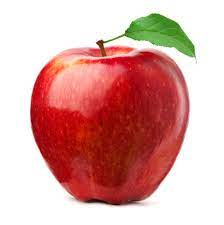
\includegraphics[scale=0.75]{../data/index.jpeg}
    %TC:ignore
    \caption{this is a photo of an apple }
    %TC:endignore
    \end{figure}

    \section*{Discussion}

    reminder of aims
    tie together results / key findings
    give results broader context - implications
    add more referencing
    what do we know now that we didnt before
    what is the chain of logic and results that means we know it (remember not to repeat anything from results section)
    extent to which original aims have been satisfied
    discuss limitations of my study and future work to address limitations
    what would i do differently if i had more time
    conclude emphasising how this study in this system is of interest to people who work on other things, or other systems

    \bibliographystyle{plain}

    \bibliography{ReportBiblio}
\end{document}